\subsection{App Implementation}
As mentioned, we chose to use the React framework to implement the user interface. That allowed us to split our code up into reusable \textit{'components'} as well as react to state changes, like update the list of contacts whenever a new contact was added, automatically.

** SHOW EXAMPLE COMPONENT **
\insertcodeblock{code/app/src/components/BatteryIndicator/BatteryIndicator.tsx}{0}{10}

To get started, we implemented a basic framework for navigating between pages in the app. It needed to support two different views discussed in the design section. Instead if importing some larger framework to do this simple task, we chose to implement a simplified version ourselves. It uses two dictionaries, one for each view, and then each key value pair corresponds to a different page in that view. Then we just keep track of the view and page that the user is on, and update the variables used to index the dictionaries when we want to navigate between pages.


\subsubsection{Database Connection}

The database is setup in a way where a collection can have a number of documents, and a document can have a set of collections and so on. A single document can then be referenced with a \textit{'reference'} (see \autoref{fig:database-reference}). A reference is just a type of file path, describing what collection, what document and so on. 

\begin{figure}[H]
    \centering
    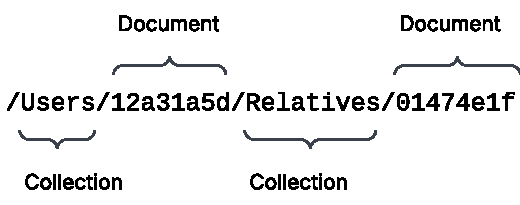
\includegraphics[width=0.5\linewidth]{report/images/Database Reference.pdf}
    \caption{Example reference}
    \label{fig:database-reference}
\end{figure}

Behind the scenes, the documents, collections and their references between could be visualized like the following (see \autoref{fig:database-diagram})

\begin{figure}[H]
    \centering
    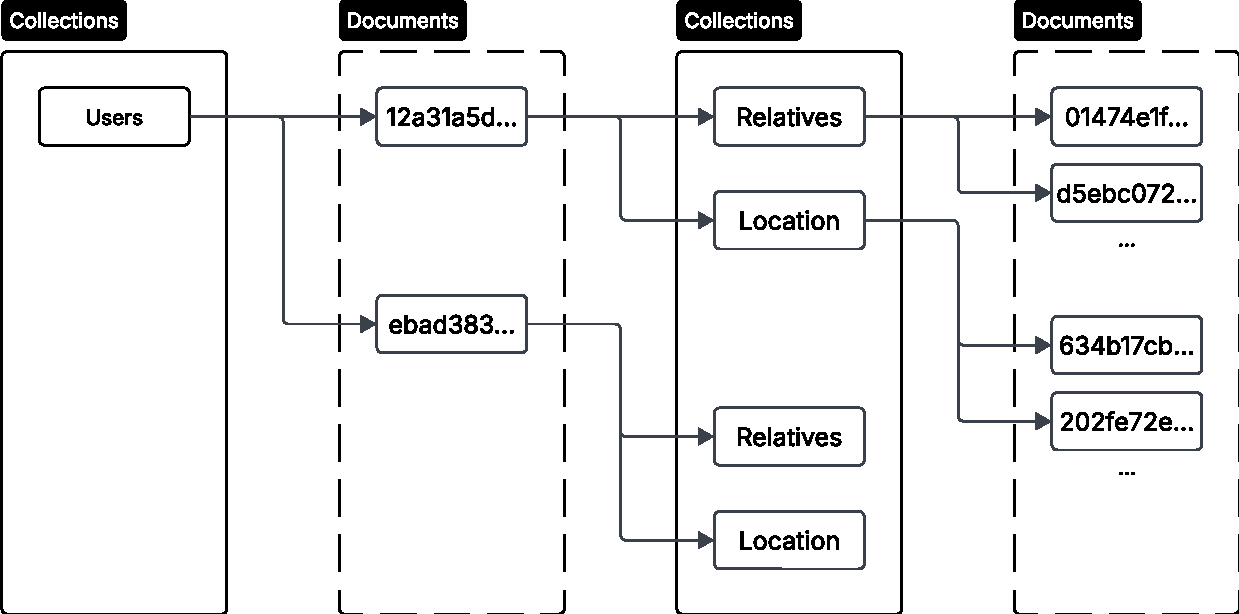
\includegraphics[width=\linewidth]{report/images/Database Diagram.pdf}
    \caption{Database Diagram}
    \label{fig:database-diagram}
\end{figure}

Here we can see a simplified example of how our database is setup. Where each user has two collections, one for their relatives, and one for their location history.

Getting and storing data in the database was quite easy due to the large community support around the Firebase ecosystem. There were existing \textit{'plugins'} for capacitor that would take advantage of the native system that the app was running on to improve the performance and usability of the plugin. One of theese plugins was meant for the Firebase Firestore database, and allows for subscribing to changes in the database, as well as regular getting, setting and deleting of documents.


\subsubsection{Bluetooth Connection}
- Scanning for new devices to pair
- Store paired devices for fast reconnect
- Alert user when disconnected

** Insert screenshot of the bluetooth connection page here

\subsubsection{\gls{gps} updates}
To allow allow the relatives to see a history of where they have been, we need to capture the location of the device, even when the user has the app in the background. This presented some challenges, as most native systems won't allow permanent location tracking due to battery consumption and privacy concerns. The real solution would be to move the \gls{gps} module to the wristband, as that would increase the precision of the location if eg. the user was in their garden and the app reported the location to be indoors, as that was where they left their phone. Due to the prototype nature of our current solution, it was the easiest to just use the \gls{gps} from the device, as that still provides a general idea of where the user is located.

Both Android and iOS have luckily thought of this, and provides a way to listen for gps updates natively. It wakes up a small part of the app to handle the update, giving us just enough time to upload it to our database to display to the relatives.

** Insert screenshot of the guardian map page here ** 

- Pushes the gps coordinates, accuracy and timestamp to a document in the database
